
\section{Map-Erkennung [H]}
Nachdem der Spieler der Lobby beigetreten ist, wird es Zeit für ihn die Spielumgebung zu zeichnen und diese für die
Abstimmung freizugeben. Das passiert indem dieser einen QR-Code (``Quick Response''), welcher sich in der
Mitte der Lobby befindet, mit einem mobilen Endgerät, welches über eine Kamera verfügt, abscannt. Somit wird
er auf eine Webseite geleitet, welche wieder auf die Kamera zugreift. Auf dieser ist bereits eine Objekterkennung
vorprogrammiert. Auf die Funktionsweise und auf die technische Umsetzung wird im folgenden \dots eingegangen. Wenn der Spieler
merkt, dass die Objekterkennung das Blatt erkannt hat, kann dieser ein Bild aufnehmen. Im nächsten Schritt ist es nochmals möglich
die erkannten Kanten zu verschieben. Wenn sich der User für das Foto als Map entscheidet kann er den ausgewählten Teil in eine
top-down-2d-Perspektive
umwandeln. Kurzgesagt werden dabei die vier ausgewählten Ecken, welche über die Kanten des Blatt Papiers liegen,
für eine Perspektiven-Transformation
mit OpenCV2 herangezogen. Wenn der Spieler dann so weit ist, kann er dieses Bild beziehungsweise diese Map bestätigen und
sendet sie somit zurück an die Lobby. Dann kann die Abstimmung beginnen.

\begin{figure}[H]
    \centering
    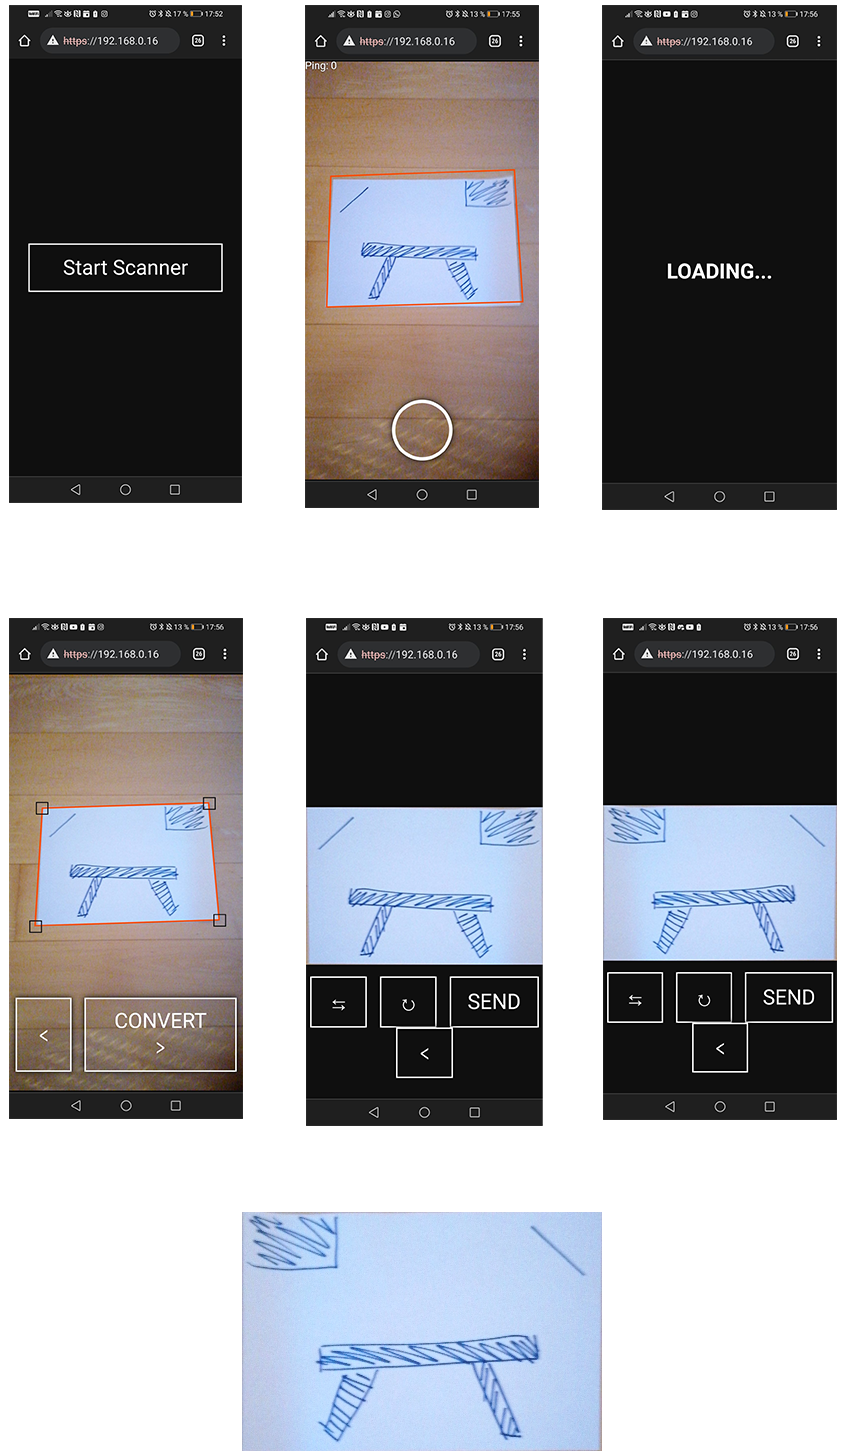
\includegraphics[scale=0.4]{pics/demo_maperkennung/sammlung_1.png}
    \caption{Screenshots der Maperkennungsanwenung}
    \label{fig:map:maperkennungsprozess}
\end{figure}

\setauthor{Himmetsberger Jonas}
\subsection{Objekterkennung [H]}
Das Thema ``Objekterkennung'' ist ein extrem schnell wachsendes und sich verbesserndes Feld in der Welt der Bildverarbeitung beziehungsweise
Bildanalyse. \\
Die Objekterkennung ist ein großer Teil der Arbeit. Hier wird aus dem live Footage der Kamera das Blatt Papier und anschließend
in einer fertigen Aufnahme die Map erkannt.
\\
\\
Die Objekterkennung wird zum Beispiel bei komplexen und großen Paketdiensten eingesetzt. Sollen Pakete nach Farbe gruppiert werden, so
reicht bereits ein Farbsensor. Das ist in den meisten Fällen jedoch nicht genügend.
Vielmals werden Pakete auf Strichcodes oder Adressen überprüft.
Wenn also unterschieden werden muss, wo welches Paket landen soll, so ist eine Kamera nötig. Diese muss
ein genügend gut auflösendes Bild aufnehmen, dass daraus Informationen gewonnen werden können. Diese Daten müssen zur Auswertung
mathematisch beschrieben werden. Zur Übersetzung werden Verfahren, wie Kantenerkennung, Transformationen oder Größen- und Farberkennung,
aber auch künstliche Intelligenzen
eingesetzt. In dieser Arbeit wurden Kanten zur Objekterkennung herangezogen.
Die Korrektheit des Ergebnisses ist abhängig von der Korrektheit der bereitgestellten Daten und wie genau das Objekt mathematisch
beschrieben werden kann.
\\
Ein weiteres Beispiel, wo Objekterkennung eingesetzt wird, ist in
Fahrerassistenzsysteme oder autonomes Fahren. Bereits in der ersten Stufe des autonomen Fahrens (dem assistierten Fahren)
werden zur Hilfe Kameras außerhalb des Fahrzeugs angebracht. In einem Auto, welches als Stufe eins autonomes Assistenzsystem
eingestuft wird, werden diese Kameras für einen automatischen Spurhalteassistenten eingesetzt. Via Bildanalyse und Objekterkennung
werden die Linien auf der Straße erkannt. \\
In höheren Stufen ist die Objekterkennung nicht mehr wegzudenken. Es müssen Verkehrsschilder und Personen auf der Straße erkannt
werden um daraufhin entsprechen zu agieren.

Andere Beispiele:
\begin{compactitem}
    \item Gesichtserkennung, um das Smartphone zu entsperren.
    \item Qualitätskontrolle, zur Erkennung und automatischen Entfernung von kaputten oder beschädigten Teilen.
    \item Personenerkennung, um Menschenmassen zu analysieren.
\end{compactitem}

\subsubsection{Beschreibung der Funktionalität [H]}

Wie schon erwähnt kann man aus Bildern Daten erkennen. Viele Pixel bilden insgesamt ein Bild, welches wir visuell aufnehmen und in welchem wir alles Mögliche erkennen können. Jeder einzelne dieser Pixel in einem digitalen Bild enthält Informationen über die Helligkeit und über die Farbe. Der Bildpunkt setzt sich zusammen aus den Farben Rot, Grün und Blau. Aus diesen drei können alle möglichen Farben abgebildet werden.
\\
Bevor ich darauf eingehe, wieso wir uns für die Konturenerkennung als Art der Bilderkennung entschieden haben, ist es noch entscheidend vorher zu wissen, wie der Mensch Objekte erkennt.
\\
In unserem Auge passiert die Farberkennung via den Zapfen. Auch hier wird die Wellenlänge des Lichts in ein Gemisch aus Rot, Grün und Blau aufgeteilt. Allerdings benötigen wir das reine Farbsehen nicht um Objekte zu erkennen. Uns reicht es schon, wenn wir nur Informationen über die Helligkeit empfinden. Somit können wir zum Beispiel auch in Schwarz-Weiß-Bildern oder in der Dunkelheit bei wenig Licht Objekte erkennen. Wir erkennen einen Unterschied zwischen Objekten, welche sich in einem dreidimensionalen Raum befinden leicht, indem das eine Objekt sich in der Helligkeit von dem anderen Objekt unterscheidet. Das heißt, dass wenn z.B. ein Würfel auf einem Boden liegt, dann erkennen wir den Würfel, weil dieser anders viel Licht reflektiert als der Boden. Und an der Stelle, wo der Würfel aufhört, erkennen wir eine Kontur. Hier ist der Unterschied zwischen Boden und Würfel erkennbar.
\\
Und genau so passiert auch die Objekterkennung in unserem Spiel ScribbleFight. Hier wird zuerst aus der Live-View, welche vom Client zur Verfügung gestellt wird, das Farbbild in Graustufen konvertiert. Das passiert, indem für jeden Pixel ein ``Durchschnitt'' der Helligkeit von allen drei Farbwerte (Rot, Grün, Blau), welche in einem 8-Bit System von 0 bis 255 geht, gebildet wird. Wie dies jedoch genauer funktioniert, wird im Kapitel Bildverarbeitungsalgorithmen
\ref{maai:alogs}
genauer erklärt. Nachdem das Bild in ein Schwarz-Weiß-Bild umgewandelt wurde, muss vor der Konturenerkennung noch ein Schwellwert-Bild erzeugt werden. In der Untenstehenden Abbildung %\ref{}% 
das dritte Bild von links.



Code stücke noch einbauen


Welche Abfolge von CV2 Bildverarbeitungsalgorithmen haben zum ergebnis geführt
noch nicht auf die Algorithmen näher eingehen
\subsection{Open-CV2 [H]}
\subsubsection{Bildverarbeitungsalgorithmen} \label{maai:alogs}
auf die algos näher eingehen
\subsubsection{Umwandlung der Bilder in für das Spiel brauchbare Daten [H]}

\begin{lstlisting}[language=Python,caption=Bild in Spielbare Map umwandeln,label=lst:umsetzung:getplayablearray]
    def getPlayableArray(img):
        np.set_printoptions(threshold=sys.maxsize)

        alpha_img = cv2.cvtColor(img, cv2.COLOR_BGR2BGRA)  # rgba
        imgWarpGray = cv2.cvtColor(alpha_img, cv2.COLOR_BGR2GRAY)
        blurred = cv2.GaussianBlur(imgWarpGray, (7, 7), 0)
        imgAdaptiveThre = cv2.adaptiveThreshold(
            blurred, 255, cv2.ADAPTIVE_THRESH_GAUSSIAN_C, cv2.THRESH_BINARY_INV, 7, 2)
        imgAdaptiveThre = cv2.bitwise_not(imgAdaptiveThre)
        imgAdaptiveThre = cv2.medianBlur(imgAdaptiveThre, 3)

        # make image square
        imgAdaptiveThre = np.array(makeSquare(
            cv2.cvtColor(imgAdaptiveThre, cv2.COLOR_BGR2BGRA)))

        img = cv2.cvtColor(imgAdaptiveThre, cv2.COLOR_BGR2BGRA)

        # pippoRGBA2 = Image.fromarray(np.array(img).astype('uint8'), mode='RGBA')
        # pippoRGBA2.show()
        cv2.imwrite(
            './source/prototypes/streamFusion/output/imgAdaptiveThre.png', imgAdaptiveThre)

        iar = np.asarray(img).tolist()

        rows = len(iar)
        columns = len(iar[0])

        meshes = 3025
        # percent = perc(rows * columns)
        percent = 95
        n = math.ceil(np.sqrt(rows * columns / meshes))
        x = 0
        y = 0

        newImg = []

        while y < rows:
            newImg.append([])
            while x < columns:

                i = 0
                j = 0
                bg = 0
                while i < n:
                    while j < n:
                        if (y + j) < rows and (x + i) < columns:
                            if np.all(iar[y + j][x + i][:3] == [255, 255, 255], 0):
                                bg += 1
                        else:
                            bg += 1
                        j += 1
                    j = 0
                    i += 1

                bgPercent = bg / (n**2)
                if (bgPercent < (percent / 100)):
                    newImg[int(y / n)].append([0, 0, 0, 255])
                else:
                    newImg[int(y / n)].append([255, 255, 255, 0])

                x += n
            x = 0
            y += n

        iar = np.asarray(newImg).tolist()
        with open('./source/prototypes/streamFusion/output/mapArray.txt', 'w') as f:
            f.writelines(repr(iar))

        # pippoRGBA2 = Image.fromarray(np.array(newImg).astype('uint8'), mode='RGBA')
        # pippoRGBA2.show()
        cv2.imwrite(
            './source/prototypes/streamFusion/output/newImg.png', np.array(newImg))

        return newImg

\end{lstlisting}
\subsection{Kommunikation mit der Lobby via Flask und Flask SocketIO [H]}

\section{KI [H]}
Im Laufe der Ausarbeitung der Diplomarbeit und der damit zusammenhängenden Forschung änderte sich oft die
Vorstellung darüber, wie das Endprodukt (KI) auszusehen hat, beziehungsweise, wie dieses aussehen kann.
Limitierungen, welche vor der Forschung noch nicht bekannt und bewusst waren, begrenzten die Lernfähigkeit der KI.
Auf Probleme, Lösungen und Ergebnisse wird jedoch noch näher in ... eingegangen.
\subsection{Lernen mit OpenAI-Gym [H]}
% \subsection{Künstliche Intelligenz Definition [H]}
\subsection{Reinforcement Learning [H]}
\subsection{Die ScribbleFight-KI [H]}
\subsubsection{Beschreibung der Funktionalität [H]}
\subsubsection{Warum Python? [H]}
\subsection{Tensorflow und Keras [H]}
\subsubsection{Tensorflow [H]}
\subsubsection{Keras [H]}
